% DO NOT COMPILE THIS FILE DIRECTLY!
% This is included by the other .tex files.

\begin{frame}
\titlepage
\end{frame}

\begin{frame}
  \frametitle{whoami}
  \begin{itemize}
    \item Iklódy András
    \item CIRCL operator
    \item 2012 óta vezetem a MISP core fejlesztését
  \end{itemize}
\end{frame}

\begin{frame}
  \frametitle{Kik is vagyunk mi - CIRCL, MISP}
  \begin{center}
    
\includegraphics[scale=0.45]{pics/circl.png}
    \hspace{2.5em}
    
\includegraphics[scale=0.35]{pics/misp.pdf}
  \end{center}
  \begin{itemize}
    \item {\bf CIRCL} - a luxemburgi állami, privát-szektorért felelős CERT
    \item Gazdasági minisztérium finanszíroz minket, hogy a Luxemburgban honos cégeknek segítsünk mindennel ami cyber-security témakörbe esik
    \item Illetve, hogy toolokkal és információval lássuk el a közösséget
    \item Mi állunk javarészt a {\bf MISP-project} mögött is, illetve aktívan megosztunk threat intelligence-t a közösséggel MISPen keresztül
  \end{itemize}
\end{frame}

\begin{frame}
  \frametitle{Megosztó közösségek}
  \begin{itemize}
    \item Feladatköreink közé tartozik különböző {\bf megosztó közösségek üzemeltetése}
    \item Illetve résztvevői vagyunk mások által üzemeltetett közösségeknek
    \item Mindenekelött {\bf napi teendőinkhez nélkülözhetetlen eszköz a MISP}
    \item Egyben mi vagyunk a {\bf fő fejlesztői} is a toolnak, de ugyanakkor az egyik legnagyobb {\bf felhasználói is}
    \item A sokféle közösségnek mind {\bf más igényei és elvárásai} vannak
  \end{itemize}
\end{frame}

\begin{frame}
  \frametitle{A prezentáció céljai}
  \begin{itemize}
    \item Rövid MISP bevezető
    \item Különböző community-k bemutatása
    \item Tapasztalatok, kihívások, kudarcok, tippek
  \end{itemize}
\end{frame}

\begin{frame}
  \frametitle{Mi is az a MISP?}
  \begin{itemize}
     \item Threat intelligence sharing platform (TISP)
     \item {\bf Open-source} és ingyenes
     \item {\bf Threat-intel begyűjtése} saját incidensekből, partnerektől, feedekből
     \item {\bf Harmonizálása és korrelációja} az adatoknak
     \item {\bf Kollaborácio} partnerekkel, áldozatokkal illetve az ügyészséggel koordinálás, stb
     \item {\bf Automatikus védelem} építése, partnerek {\bf informálása}, stb
  \end{itemize}
\end{frame}

\begin{frame}
  \frametitle{Milyen jellegű közösségeket üzemeltetünk?}
  \begin{itemize}
    \item Általános megosztó közösség a privát szektornak
    \begin{itemize}
      \item 1200 szervezet és 3500 felhasználó
      \item {\bf Általános központi hub}, különböző közösségek összecsatolása
      \item {\bf Cégek, CERT-ek, SoCok, kutatók}, a világ minden részéről
      \item Ekkora community építése {\bf időbe telik} (éves növekedés):
    \end{itemize}
  \end{itemize}
  \begin{center}
      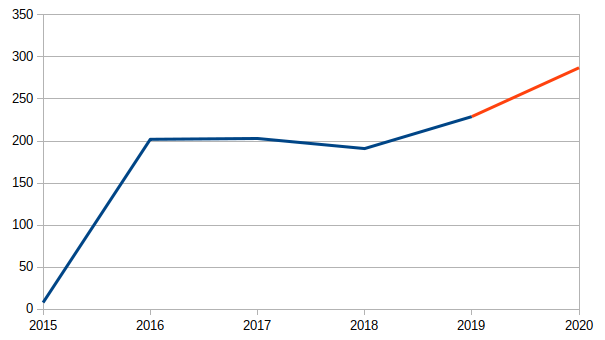
\includegraphics[scale=0.5]{pics/org_growth.png}
  \end{center}

\end{frame}

\begin{frame}
  \frametitle{Milyen jellegű közösségeket üzemeltetünk?}
  \begin{itemize}
    \item {\bf Nemzeti} illetve {\bf katonai CERT}ek community-jei
    \item {\bf Regionális és szektoriális} ISAC-ek MISP közösségei
    \item Különböző {\bf témakörökkel} foglalkozó közösségek (pl GSM, financial fraud, stb)
    \item Röviden: sokféle közösség létezik, van, amelyik sikeresebb, van amelyik kevésbé
  \end{itemize}
\end{frame}

\begin{frame}
  \frametitle{Egy új közösség létrehozása}
  \begin{itemize}
      \item A technikai kivitelezés nagyon egyszerű
      \item Egy {\bf központi MISP server telepítése} elegendő a folyamat megindításához, ezt bárki megteheti
      \item Első lépésben a partnereink használhatják a mi MISP-ünket
      \item Ha idővel növekedni akarnak, {\bf saját MISPet telepíthetnek es összeköthetik} a miénkkel
      \item De az igazi kihívás nem ebben van
  \end{itemize}
\end{frame}

\begin{frame}
  \frametitle{Közösségi célok és elvárások}
  \begin{itemize}
      \item Akárhogy is nézzük, maga az információ elkészítése mindig is {\bf időigényes} lesz
      \item Első lépés: {\bf elérhető és egyértelmű célok és szabályok} felállítása
      \begin{itemize}
          \item Milyen információ {\bf releváns} az adott csoportnak?
          \item {\bf Kiket} akarunk felvenni a tagok közé (Szektor? Régió? ISAC? NGOk? Technikai képességek?)
          \item Milyen {\bf szótárakat} használjunk az adatok {\bf kontextualizálásához}?
          \item Mit csinálhatunk az adatokkal, amiket megosztunk?
      \end{itemize}
  \end{itemize}
\end{frame}

\begin{frame}
  \frametitle{Játekszabályok}
  \begin{itemize}
      \item Ha túl sok a feltétel, {\bf elijesztjük a usereinket}
      \item 20 oldalas jogi szöveg helyett pár mondatba foglalt szabályok
      \item A cél: első ránézésre tudjuk, hogy valamit megoszthatunk-e
      \item Készüljünk fel: A jogi csapatunk elsőre valószínűleg meg fog ijedni az ötlettől
      \begin{itemize}
          \item Mi van, ha túl sokat osztunk meg?
          \item Jogi alapja a megosztásnak (compliance dokumentumok: https://github.com/CIRCL/compliance)
      \end{itemize}
      \item Procedúrák felállítása {\bf anonym megosztáshoz}
  \end{itemize}
\end{frame}

\begin{frame}
  \frametitle{Adatok struktúrálása}
  \begin{itemize}
      \item Milyen kifejezéseket használjunk {\bf kontextualizálásra}?
      \item Taxonómiák kiválasztása, létrehozása
      \item {\bf IoC listák vs komplex kontextualizált gráfok}
      \item {\bf IoC lifecycle management}
      \item A legfontosabb: {\bf Imitáció} - első prioritás a helyes content gyártása
  \end{itemize}
\end{frame}

\begin{frame}
  \frametitle{Adatok struktúrálása}
  \begin{center}
    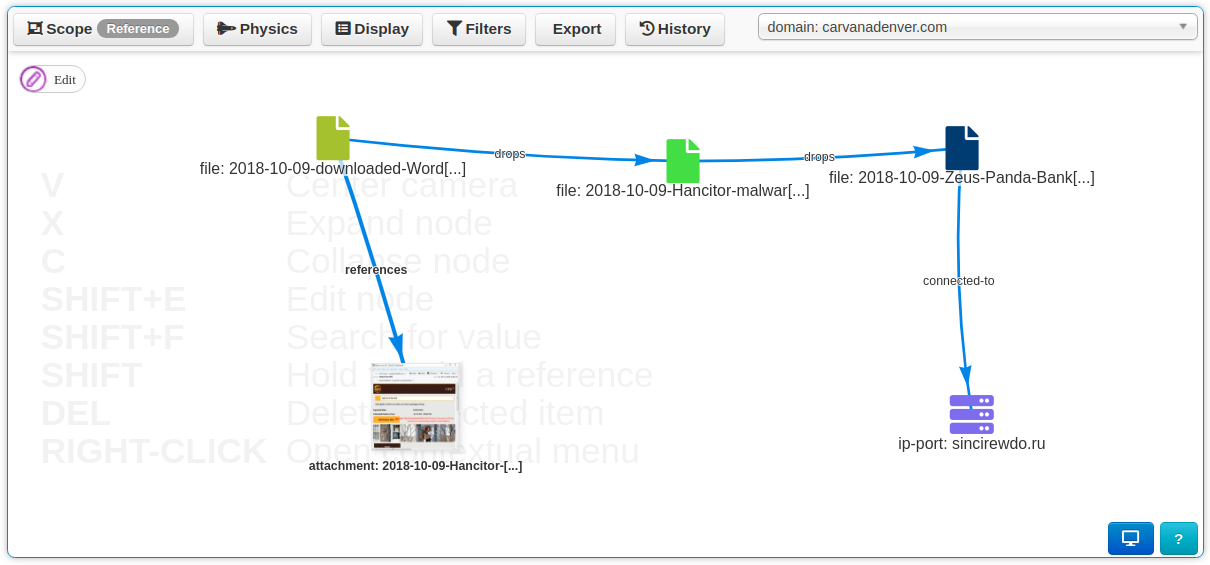
\includegraphics[scale=0.3]{pics/eventgraph.png}
  \end{center}
\end{frame}


\begin{frame}
  \frametitle{Legyünk befogadóak}
  \begin{itemize}
      \item {\bf Homogén közösségek nem léteznek}
      \item Különböző technikai fejlettség, csapat méretek, igények, use-case-ek, megosztási akarat
      \item Ezek a tulajdonságok {\bf idővel változnak}, ha valakit kirekesztünk késöbb lehet, hogy megbánjuk
      \item Fogadjuk el a különbségeket és használjuk előnyként
      \item Ha egy szervezet csak felhasználja az adatainkat és nem ad vissza semmit a közösségnek, az is lehet előny
  \end{itemize}
\end{frame}

\begin{frame}
  \frametitle{Legyünk befogadóak}
  \begin{itemize}
      \item Egy {\bf fejlettebb, összetartó közösség minket is véd}, javítsunk a helyzeten:
      \begin{itemize}
          \item Workshopok, trainingek
          \item Összejövetelek
          \item Kommunikációs csatornák
      \end{itemize}
  \end{itemize}
\end{frame}

\begin{frame}
  \frametitle{Kudarcok}
  \begin{itemize}
      \item Az első próbálkozásunk: Bomba-biztos {\bf Terms and Conditions}
      \item Üres megosztó közösségek
      \item Megosztási {\bf kvóták}
      \item Emberi {\bf tévedések} kezelése
      \item {\bf Kitartás} hiánya (ellenpélda, CIRCL privát szektor):
      \begin{itemize}
         \item Szervezetek: 1214
         \item Legalább egy "event" létrehozása: 160
         \item Átlagos idő első megosztásig: 210 nap
      \end{itemize}
      \item Adjuk meg a {\bf kellő elismerést} azoknak, akik megosztanak információt
  \end{itemize}
\end{frame}

\begin{frame}
  \frametitle{De hogyan is vegyük rá a közösségünket az aktiv megosztásra?}
  \begin{itemize}
      \item Organikus növekedés
      \item {\bf Mindenki önző} - és ez nem feltétlenül probléma
      \item A legfontosabb kérdés - {\bf milyen threat intel a legfontosabb a szervezetünknek}?
  \end{itemize}
  \begin{center}
    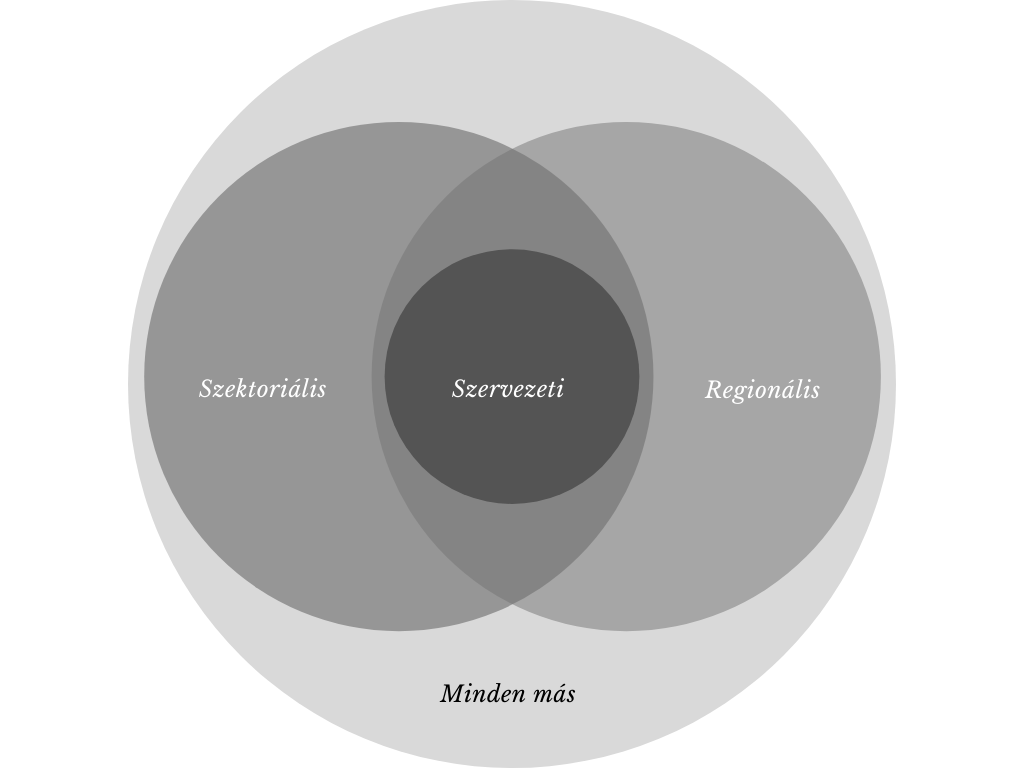
\includegraphics[scale=0.2]{pics/informacio-forrasok.png}
  \end{center}
  \begin{itemize}
      \item Visszajelzés, kollaboráció a saját incidenseknél
  \end{itemize}
\end{frame}

\begin{frame}
  \frametitle{Konklúzió}
  \begin{itemize}
      \item Röviden láttuk, {\bf miről szól a MISP}
      \item Azt is, hogy egy megosztó {\bf közösség létrehozása egyszerű}
      \item De ahhoz, hogy sikeres is legyen, fontos az {\bf átgondolt community management}
      \item Illetve még fontosabb a {\bf kitartás és a pozitív hozzáállás}
  \end{itemize}
\end{frame}

\begin{frame}
  \frametitle{Kapcsolat}
  \begin{itemize}
    \item Iklódy András
    \begin{itemize}
      \item \url{https://twitter.com/iglocska}
      \item andras.iklody@circl.lu
    \end{itemize}
    \item CIRCL
    \begin{itemize}
      \item info@circl.lu
      \item \url{https://twitter.com/circl_lu}
      \item \url{https://www.circl.lu/}
    \end{itemize}
    \item MISPProject 
    \begin{itemize}
      \item \url{https://github.com/MISP}
      \item \url{https://gitter.im/MISP/MISP}
      \item \url{https://twitter.com/MISPProject}
    \end{itemize}
  \end{itemize}
\end{frame}
